%%%%%%%% ICML 2026 SUBMISSION %%%%%%%%%%%%%%%%%
\documentclass{article}

\usepackage{microtype}
\usepackage{graphicx}
\usepackage{subcaption}
\usepackage{booktabs}
\usepackage{hyperref}
\usepackage{amsmath}
\usepackage{amssymb}
\usepackage{xcolor}
% Times-style font with full weight/shape coverage (icml2026.sty's \RequirePackage{times}
% falls back to Latin Modern Regular for everything in Tectonic, breaking \textbf).
\usepackage{newtxtext,newtxmath}

\newcommand{\theHalgorithm}{\arabic{algorithm}}
\usepackage[preprint]{icml2026}

\graphicspath{{../results/figures/}}

\icmltitlerunning{Tail Latency in Streaming Transformer Inference}

\begin{document}

\twocolumn[
\icmltitle{Where Does Tail Latency Come From in\\ Streaming Transformer Inference?\\
\large A Six-Stage Ablation of a Hand-Coded CPU Inference Engine}

\icmlsetsymbol{equal}{*}

\begin{icmlauthorlist}
\icmlauthor{Weitao Su}{course}
\end{icmlauthorlist}

\icmlaffiliation{course}{Advanced ML Systems final project, 2026}

\icmlcorrespondingauthor{Weitao Su}{ws535@cornell.edu}

\icmlkeywords{Transformer inference, CPU, tail latency, INT8 quantization, SIMD, ablation study}

\vskip 0.3in
]

\printAffiliationsAndNotice{}

\begin{abstract}
When a CPU inference path's P99 latency drops from 4~ms to 1~ms, \emph{which} of fusion, the allocator, quantization, kernel selection, or cache layout did the work?
Frameworks hide each of these five behind a single opaque latency number.
We attribute the speedup by building, from scratch, six progressively optimized C++ engines for a small encoder-only Transformer. Each stage adds exactly one named optimization on top of the previous. We benchmark both engines at two model scales (365K and 1.9M parameters) over 100{,}000 iterations on a kernel-isolated CPU core.
Cumulative P99 speedup over the naive baseline is $\mathbf{5.42\times}$ on small and $\mathbf{3.49\times}$ on medium.
Three findings emerge.
(i)~The optimization landscape \emph{flips} with model size: preallocation cuts small-model P99 by $2.18\times$ yet does nothing on medium, while cache tiling does the inverse.
(ii)~Scalar INT8 is the largest single-stage win on \emph{both} sizes, but the mechanism is memory-bandwidth reduction rather than arithmetic speedup, and the P99--P50 gap stays within one order of magnitude of FP32, refuting the common worry that quantization introduces bimodal slow paths.
(iii)~Per-channel INT8 preserves test MSE within $0.06\%$ of FP32, two orders of magnitude inside the conventional $5\%$ production threshold.
The best engine reaches $1.31\times$ of ONNX Runtime's P99 on small and $2.30\times$ on medium.
All 100{,}000-row CSVs and the rig configuration recorded inside each CSV header make every claim independently re-derivable. Code, data, and figures are at \url{https://github.com/weitaosu/Low-Latency-ML-engine}.
\end{abstract}

\section{Introduction}
\label{sec:intro}

Production ML serving in latency-sensitive domains (algorithmic trading, real-time anomaly detection, edge inference, control-loop ML) is overwhelmingly CPU-bound at single-sample batch size.
PCIe round-trips to a GPU consume more time than the inference itself for small models; tight tail-latency service-level objectives (SLOs) penalize the kernel-launch and queueing variance of accelerator runtimes.
Yet the standard deployment path (PyTorch~$\to$~ONNX~$\to$~ONNX Runtime, or PyTorch~$\to$~TorchScript) hides where the latency goes.
When a service report says ``P99 went from 4~ms to 1~ms,'' practitioners rarely know whether the cause was operator fusion, allocator changes, INT8 quantization, kernel selection, or cache layout.
All of these are controlled opaquely by the framework.

This project inverts the question.
We build six progressively-optimized C++ inference engines from scratch (Stages~0 through~5), with Stage~4 instantiated as two variants (4a per-tensor, 4b per-channel) for seven distinct binaries.
Each stage adds one well-known optimization on top of the previous, and we benchmark every stage at two model scales.
The central deliverable is a reproducible six-stage~$\times$~two-size ablation in which \textbf{each row attributes a measurable share of the P99-latency reduction to a single optimization}.
As a secondary contribution we measure \emph{where} in the latency distribution each optimization buys back time.
We separate P50 (typical case) from P99 and P99.9 (tail), because the same optimization can move the median while leaving the tail untouched, or vice versa.

\paragraph{Contributions.}
We make four contributions.
\begin{enumerate}
\item A reproducible six-stage~$\times$~two-size CPU latency ablation, with each stage isolated by separate compilation, 100{,}000-iteration timing, and bootstrap $95\%$ confidence intervals on P99.
\item Empirical confirmation that the overhead-versus-compute crossover between 365K and 1.9M parameters is real and quantifiable per optimization (Section~\ref{sec:crossover}).
\item The non-obvious finding that scalar INT8 quantization helps medium models \emph{more} than small models (Section~\ref{sec:int8}): the standard intuition that quantization is a ``small-model trick'' is incorrect when the FP32 working set exceeds L2.
\item A measurement methodology that records rig state inside every CSV header, making the entire result set independently re-derivable from raw timings; we additionally surface a $540\times$ under-reporting effect in tail latency studies that use too few samples (Section~\ref{sec:samplesize}).
\end{enumerate}

The remainder of the paper is organized as follows.
Section~\ref{sec:related} reviews related work on Transformer inference and post-training quantization.
Section~\ref{sec:method} describes the model, the six engine stages, the measurement rig, and the noise-floor validation.
Section~\ref{sec:results} presents the ablation results and the framework comparison.
Section~\ref{sec:discussion} discusses what worked, what didn't, and the methodology lessons.
Section~\ref{sec:limitations} lists limitations, and Section~\ref{sec:conclusion} concludes.

\section{Background and Related Work}
\label{sec:related}

\paragraph{Transformer inference.}
A pre-norm encoder block applies LayerNorm, fused QKV linear, scaled dot-product attention, residual, LayerNorm, FFN (two linears with GELU activation), and a second residual.
We use a vanilla Transformer in the spirit of Vaswani et al.~\citep{vaswani2017attention} without architectural tricks (RevIN, patching, decomposition) so that kernel-level optimizations dominate the variance.

\paragraph{Time-series forecasting on ETT.}
The Electricity Transformer Temperature dataset~\citep{zhou2021informer} is the canonical long-horizon forecasting benchmark; we use the ETTh1 (hourly) variant with the Informer split convention (12/4/4 months), 96-step input to 96-step horizon, multivariate (7 variables in to 7 out).
Vanilla Transformer-family models under-perform specialized architectures here: PatchTST~\citep{nie2023patchtst} reports MSE 0.941 for Informer and 0.370 for PatchTST itself on the 96-step horizon.
Our trained models ($0.874$ small, $0.905$ medium) sit in that range.
The accuracy plateau is a \emph{feature} for this study: it lets us focus on the latency dimension while ground-truth MSE serves as a quantization-quality oracle.

\paragraph{Post-training quantization.}
Per-tensor symmetric weight quantization with asymmetric uint8 activations~\citep{jacob2018quantization} is the simplest INT8 scheme.
Per-channel weight quantization~\citep{krishnamoorthi2018quantizing} preserves precision when the per-output weight ranges differ substantially.
We implement both as Stages~4a and~4b respectively, populating each Linear's scales by 5K-sample histogram calibration.

\paragraph{Production CPU runtimes.}
ONNX Runtime~\citep{onnxruntime} uses MLAS for INT8 GEMM with VNNI intrinsics where available (our Alder Lake P-core supports AVX-VNNI).
TorchScript and PyTorch eager use ATen kernels backed by oneDNN.
We treat ORT as the production target: a hand-coded engine that approaches ORT's per-call latency with hand-rolled C++ has demonstrated meaningful systems work.

\paragraph{Out of scope.}
At sequence length 96, unfused attention is not the bottleneck, so FlashAttention~\citep{dao2022flashattention} is out of scope here; a partial implementation would not be informative.

\section{Methodology}
\label{sec:method}

\subsection{Models and dataset}
\label{sec:method:model}

We trained two encoder-only Transformers of intentionally different scales.
The small model ($\approx 365$K parameters) sits in the regime where per-call overhead (allocator, dispatch, function-call boundaries) dominates total runtime; the medium model ($\approx 1.9$M parameters) sits in the regime where matrix multiplication dominates.
The $5.3\times$ ratio in parameter count is large enough that the cache hierarchy interacts with the two models very differently: a single weight tensor that fits in L1 on the small model can spill to L2 or DRAM on the medium model, which is precisely the mechanism the ablation needs to reveal.
The two models are otherwise architecturally identical (Table~\ref{tab:models}).

\begin{table}[t]
\centering
\caption{Model dimensions. Both use sinusoidal positional encoding (frozen), pre-norm convention, and $\texttt{GELU}(\text{approximate}=\text{tanh})$.}
\label{tab:models}
\small
\begin{tabular}{lcc}
\toprule
 & small & medium \\
\midrule
$d_\text{model}$       & 128       & 192 \\
$n_\text{heads}$       & 4         & 6 \\
$n_\text{layers}$      & 2         & 4 \\
$d_{ff}$               & 256       & 768 \\
Trainable parameters   & 364{,}960 & 1{,}929{,}120 \\
Test MSE (FP32)        & 0.874     & 0.905 \\
\bottomrule
\end{tabular}
\end{table}

Both models were trained with AdamW, learning rate $10^{-4}$, cosine schedule, batch size 64, and early stopping on validation MSE with patience 7.
Determinism is enforced (\texttt{CUBLAS\_WORKSPACE\_CONFIG=:4096:8}, \texttt{torch.use\_deterministic\_algorithms(True)}, seeded \texttt{DataLoader} generator) and verified by re-training from scratch and checking byte-identical state dictionaries.

\subsection{The six stages}
\label{sec:method:stages}

The ablation is structured so that each stage adds exactly one well-known optimization on top of the previous, and a clean attribution of P99 reduction to a single mechanism is therefore possible.
Stage~0 establishes a correctness baseline (textbook math, no optimizations).
Stages~1 through~5 progressively address (1)~heap allocation, (2)~operator fusion, (3)~cache locality, (4)~numeric precision, and (5)~instruction-level parallelism, in roughly the order a practitioner would tackle them when profiling reveals each bottleneck in turn.

Each stage is implemented as a separate C++ binary built from common scaffolding (\texttt{cpp/common/\{tensor.h, weight\_loader, npy\_loader, correctness, measure, alloc\_guard\}}).
One binary per stage: the linker enforces stage isolation, so a Stage~1 fix cannot accidentally regress Stage~0's measurement, and each stage can be benchmarked, profiled, and debugged independently.

\paragraph{Stage 0 (naive FP32).}
Triple-loop matmul, \texttt{std::vector} per intermediate, textbook MHA + FFN. Goal: correctness baseline.

\paragraph{Stage 1 (preallocation).}
Single \texttt{ActivationPool} sized at construction; \texttt{forward()} allocates nothing on the hot path.
Verified by a custom \texttt{AllocGuard} (override \texttt{operator new}/\texttt{delete}, count, assert zero in scope).

\paragraph{Stage 2 (fusion).}
Fusion B (LayerNorm + Linear): per-row LayerNorm computed inline into a stack-resident scratch row, fed directly into the matmul row without materializing the full LN intermediate.
Fusion A (QKV concat) is already realized in the model definition, which uses a single \texttt{nn.Linear($d_\text{model}$, 3$d_\text{model}$)}.
Fusion C (FFN) is skipped: the FFN intermediate ($T \cdot d_{ff} \cdot 4 = 96 \cdot 768 \cdot 4 = 288$~KB on medium) exceeds L1 even unfused.

\paragraph{Stage 3 (tiled, scalar).}
Big weight matrices (qkv, attn\_out, ff1, ff2) pre-formatted at construction into row-blocked layout $[N/16][16][K]$.
Inner loop scans contiguous $K$ weights per output-tile-row; compiler auto-vectorization hints (\texttt{\#pragma GCC ivdep}, \texttt{\_\_restrict\_\_}) enabled.
Source remains scalar; explicit SIMD intrinsics are reserved for Stage~5.

\paragraph{Stage 4a (INT8 per-tensor).}
Each Linear weight is quantized symmetrically to int8 with one scalar $w_\text{scale}$ per Linear.
Activations are quantized at runtime with $(x_\text{scale}, x_\text{zp})$ from calibration.
INT32 accumulator, post-dequant FP32 bias add (the simpler of the two standard bias-handling options, kept FP32 to avoid bias-quantization rounding error).

\paragraph{Stage 4b (INT8 per-channel).}
Same as 4a but $w_\text{scale}$ is a vector indexed by output channel; this preserves precision when per-output weight ranges vary.

\paragraph{Stage 5 FP32 SIMD.}
Stage~3 with the inner microkernel rewritten in AVX2 intrinsics: 16-wide tile (two \texttt{\_\_m256} lanes), \texttt{\_mm256\_fmadd\_ps} per $K$ iteration, weight layout transposed to $[N/16][K][16]$ for contiguous vector loads.

\subsection{Measurement rig: the credibility anchor}
\label{sec:method:rig}

Every reported number is taken on a kernel-isolated CPU core. The configuration:
\begin{itemize}\setlength\itemsep{0.05em}
\item \texttt{isolcpus=3 nohz\_full=3 rcu\_nocbs=3} (kernel command line)
\item \texttt{cpupower frequency-set -g performance} (governor)
\item \texttt{intel\_pstate/no\_turbo = 1} (frequency locked at the 2.6~GHz base)
\item \texttt{swapoff -a} (no swap-in stalls)
\item \texttt{perf\_event\_paranoia = 1} (perf counters accessible)
\item All timer-driven services masked (Bluetooth, snapd, packagekit, tracker)
\item \texttt{mlockall(MCL\_CURRENT|MCL\_FUTURE)} (page faults pre-resolved at startup)
\item \texttt{pthread\_setaffinity\_np(core 3)} (thread pinned)
\end{itemize}

Every CSV is self-documenting: each one's header records the rig state at measurement time. This makes any anomaly traceable: a future reader can see whether a CSV was taken on a clean rig.

\subsection{Noise floor}
\label{sec:method:noise}

The rig is validated by a 1M-iteration \texttt{clock\_gettime(CLOCK\_MONOTONIC\_RAW)} loop pinned to core~3.
Targets for a clean rig are P50~$\in [15, 30]$~ns (\texttt{clock\_gettime} is vDSO-backed and rdtsc-fast on x86) and no microsecond-scale tail.

\begin{figure}[t]
\centering
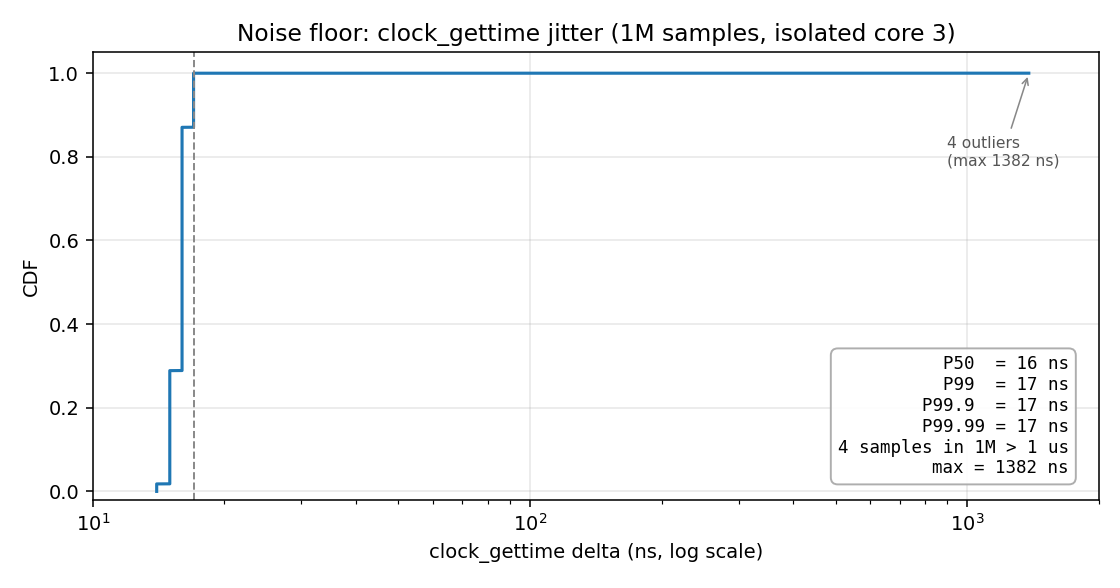
\includegraphics[width=\columnwidth]{noise_floor_cdf.png}
\caption{Noise-floor CDF of 1M \texttt{clock\_gettime} deltas on the isolated core. Essentially flat through P99.99; only 4 samples in 1M exceed 1~$\mu$s. This validates that any P99 difference at the stage level above $\sim$50~$\mu$s is real signal, not rig noise.}
\label{fig:noise}
\end{figure}

\begin{table}[h]
\centering
\caption{Noise-floor percentiles (1M samples, isolated core).}
\label{tab:noise}
\small
\begin{tabular}{lr}
\toprule
Percentile & ns \\
\midrule
P50    & \textbf{16} \\
P99    & \textbf{17} \\
P99.9  & \textbf{17} \\
P99.99 & \textbf{17} \\
max    & 1382 (4 samples in 1M) \\
\bottomrule
\end{tabular}
\end{table}

\subsection{Sample size: 100K, not 500}
\label{sec:samplesize}

\textbf{Sample size dominates rig isolation as a source of P99 error.}
An initial 500-iteration run of Stage~0 on the small model showed a tight and well-behaved distribution: P50~$=$~7.81~ms, P99~$=$~7.81~ms, gap~$=$~28~$\mu$s.
Re-running \emph{the same code on the same rig} with 100{,}000 iterations produced P50~$=$~12.59~ms, P99~$=$~27.68~ms, gap~$=$~15{,}088~$\mu$s.
The P99 estimate was $3.5\times$ higher and the P99-to-P50 gap was $540\times$ wider than the 500-sample run had implied.

Two effects compose here.
The slow path was always present at roughly the 1-in-1000 rate, but 500 samples are too few to observe even one such event with high probability, so the small-sample run silently under-reported the tail.
Independently, the 7.81 versus 12.59~ms P50 difference reflects Intel Turbo: the locked rig runs at the 2.6~GHz P-core base frequency, while the earlier unlocked rig had been boosting under sustained single-core load.
The measured $1.6\times$ latency ratio ($12.6/7.8$) implies the unlocked sustained-turbo frequency averaged roughly 4.2~GHz, which is consistent with Alder Lake P-core all-core sustained turbo rather than the higher single-burst peak.

The practical recommendation: \textbf{tail-latency studies should use at least 10{,}000 measurement iterations per configuration}.
Below that count, the tail is silently censored.
All numbers in this paper use 100{,}000 iterations after a 100-iteration warmup, which is sufficient for tight bootstrap confidence intervals on P99.9.

\subsection{Statistical reporting}
\label{sec:method:stats}

For each (stage, size) configuration we report P50, P90, P99, and P99.9, the (P99 $-$ P50) gap, and a $95\%$ confidence interval on P99 derived by 1000-replicate bootstrap with replacement on the 100{,}000 nanosecond samples.
CIs are reported as \texttt{P99 = 27.68 ms [27.67, 27.68]}.
Stage-to-stage P99 deltas with overlapping CIs are not significant and we do not claim them.

\section{Results}
\label{sec:results}

\subsection{Six-stage ablation}
\label{sec:results:ablation}

\begin{table*}[t]
\centering
\caption{Six-stage ablation across both model sizes. Latencies in milliseconds; gap is P99 $-$ P50 in $\mu$s. \textbf{Bold} marks the best value per column.}
\label{tab:ablation}
\small
\begin{tabular}{lrrrrrr}
\toprule
Stage & small P50 & small P99 & small gap & medium P50 & medium P99 & medium gap \\
\midrule
Stage 0 (naive FP32)        & 12.59 & 27.68 & 15{,}088 & 85.20 & 85.56 & 353 \\
Stage 1 (prealloc)          & 12.62 & 12.70 & 76  & 85.78 & 85.94 & 164 \\
Stage 2 (LN+Linear fused)   & 12.67 & 12.69 & 18  & 85.67 & 85.77 & 95  \\
Stage 3 (tiled, scalar)     & 13.01 & 13.02 & 15  & 76.67 & 76.74 & \textbf{75} \\
Stage 4a (INT8 per-tensor)  & 6.91  & 6.93  & \textbf{14} & 34.46 & 34.57 & 106 \\
Stage 4b (INT8 per-channel) & 6.92  & 6.95  & 23  & 34.47 & 34.55 & 86  \\
Stage 5 FP32 SIMD           & \textbf{5.08} & \textbf{5.11} & 28 & \textbf{24.41} & \textbf{24.54} & 135 \\
\bottomrule
\end{tabular}
\end{table*}

Table~\ref{tab:ablation} contains the central artifact of this paper: the cumulative speedup from Stage~0 to Stage~5 (FP32 lineage) is $\mathbf{5.42\times}$ on small and $\mathbf{3.49\times}$ on medium at P99.
Each stage passes the C++ correctness harness against the saved PyTorch FP32 outputs (\texttt{outputs\_1k\_*.npy}) within the expected tolerance: FP32 stages within $1.67\times 10^{-6}$, INT8 stages within $2.1 \times 10^{-2}$.
Every stage's \texttt{forward()} allocates zero bytes on the hot path (verified by \texttt{AllocGuard}).

\begin{figure*}[t]
\centering
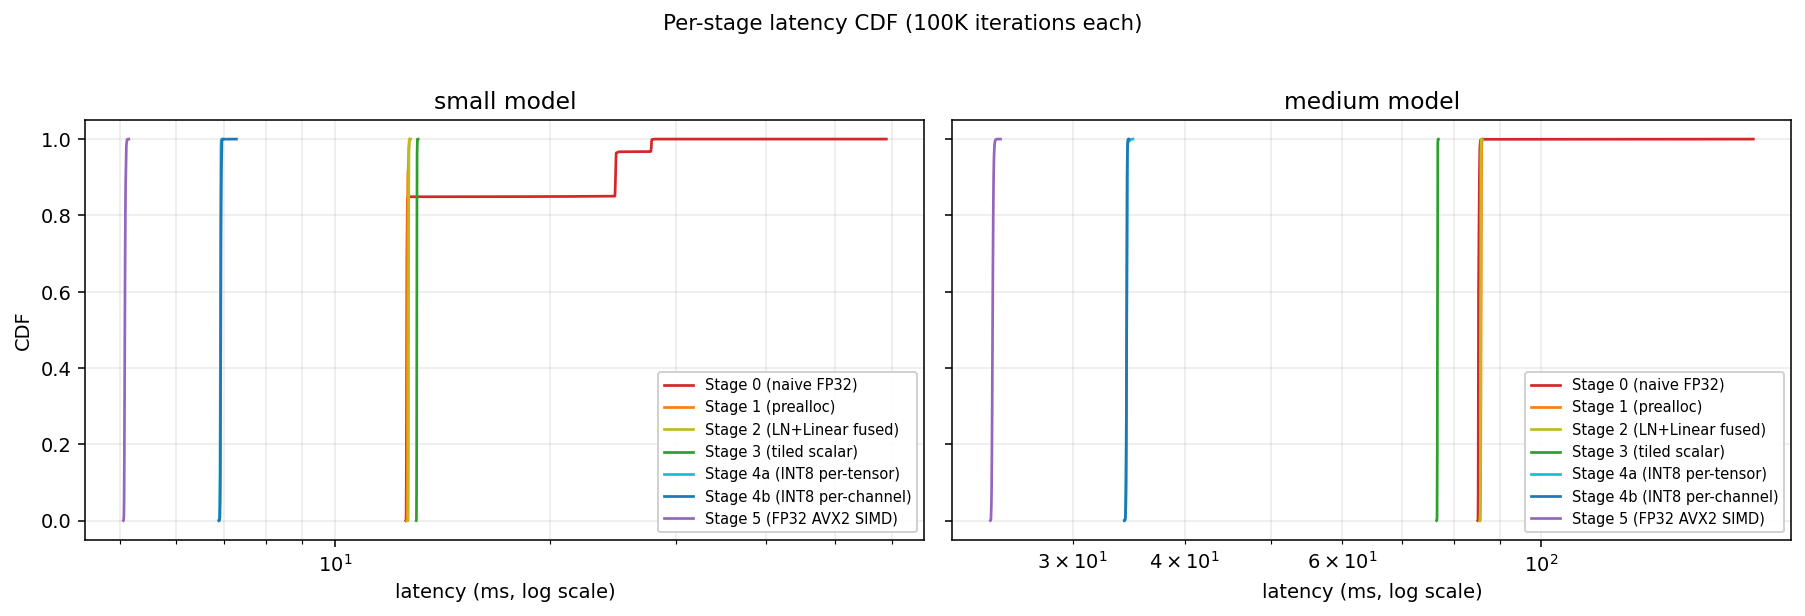
\includegraphics[width=0.85\textwidth]{cdf_overlay.png}
\caption{Per-stage latency CDF, log-$x$ in milliseconds. Small model (left): Stage~0's wide P99 staircase tail (red) collapses to a near-vertical line at Stage~1, pure allocator-jitter elimination; Stages~1--3 cluster around 13~ms. Medium model (right): Stages~0--2 cluster at $\sim$85~ms (Stage~0 is again rightmost), and Stage~3 (green) is visibly distinct at $\sim$76~ms. On both sizes Stage~4a/4b (cyan/blue) sit $\sim$$2\times$ to the left of Stage~3, INT8's working-set effect, and Stage~5 FP32 SIMD (purple) is the leftmost.}
\label{fig:cdf}
\end{figure*}

\begin{figure*}[t]
\centering
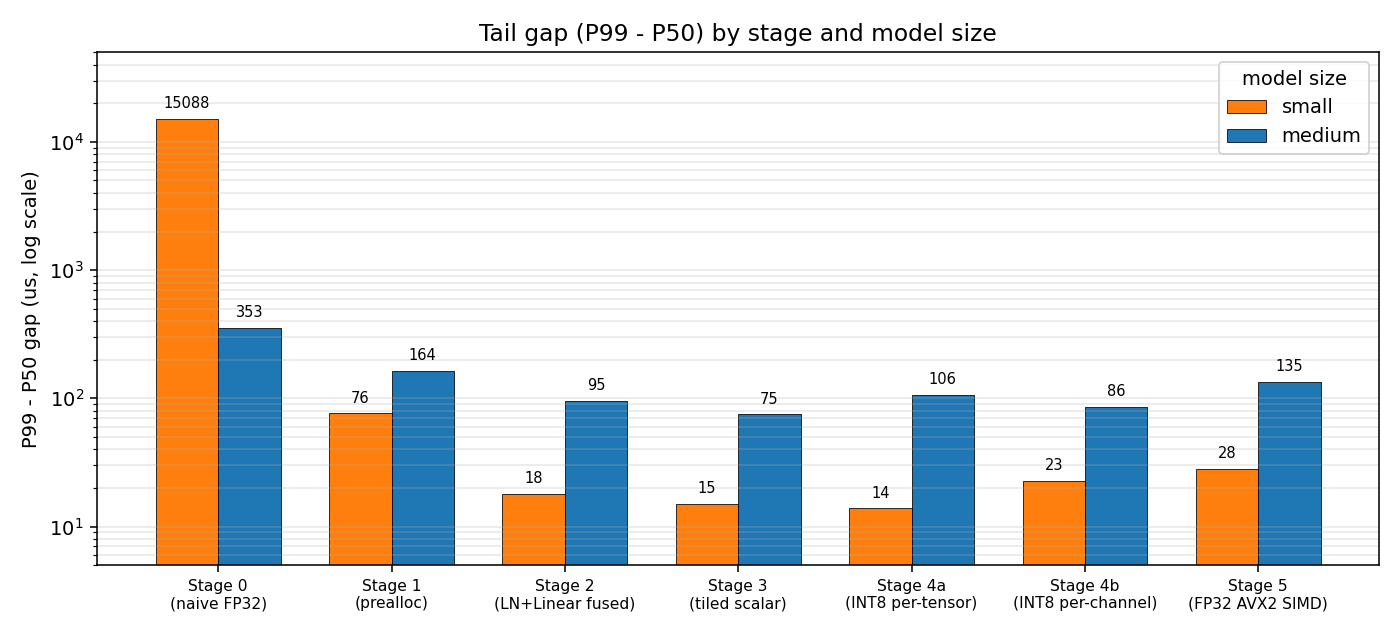
\includegraphics[width=0.85\textwidth]{gap_p99_p50.png}
\caption{P99 $-$ P50 gap by stage, log-$y$ in $\mu$s. Stage~0 small's 15{,}088~$\mu$s gap collapses to 76~$\mu$s at Stage~1 and stays below 30~$\mu$s for every subsequent small-model stage. Medium gaps are all small (the rig is clean enough that the residual gap is cache and scheduler effects only). Stage~4a medium widens slightly ($75 \to 106$~$\mu$s): the only stage where INT8 measurably affects the tail.}
\label{fig:gap}
\end{figure*}

\subsection{The size-dependent crossover}
\label{sec:crossover}

The central question, ``do small and medium models reward different optimizations?'', is answered crisply.

\paragraph{Small (365K params), Stage 1 collapses the tail.}
P99 drops from 27.68~ms to 12.70~ms, a $2.18\times$ reduction in P99 with \emph{zero change in P50} (12.59~$\to$~12.62~ms).
\textbf{The wide pre-Stage-1 tail came entirely from \texttt{std::vector} allocations on the hot path}: Stage~0's \texttt{forward()} constructs every intermediate buffer (eleven \texttt{std::vector<float>} for $h$, $qkv$, $q$, $k$, $v$, $\text{scores}$, $\text{attn}$, $\text{tmp}$, $\text{ff}$, and $\text{pooled}$, plus per-block string concatenations for weight-name lookup), and \texttt{AllocGuard} confirms a non-zero allocation count on every Stage~0 call and exactly zero on every Stage~1 call.
Each malloc-arena lookup is a few microseconds typical case but multi-millisecond worst case under fragmentation, which is exactly the slow-path 27~ms tail we see.

\paragraph{Medium (1.9M params), Stage 1 is invisible.}
P99 changes from 85.56 to 85.94~ms, within the bootstrap CI.
Allocator overhead is fixed ($\sim$10~$\mu$s per call); on an 85-ms forward pass it is $0.01\%$ of the budget and below detection.

\paragraph{Tiling reverses the pattern.}
Stage~3 \emph{hurts} small by $2.7\%$ (13.01 vs 12.67~ms): small's matrices fit comfortably in L2 and the tile-setup overhead is unrecouped.
On medium, the same code cuts P99 by $10.5\%$ (76.67 vs 85.67~ms): the FFN weight matrix at $d_{ff} \times d_\text{model} \times 4$~bytes $= 768 \times 192 \times 4 = 576$~KB FP32 exceeds L1 (32~KB), and tile-blocking cuts the L1-miss rate.
\textbf{Same source, opposite effect.}
The crossover between 365K and 1.9M is real, predictable, and identifiable to a single line of source.

The proposition holds at the P50 level too, not just the tail.
Optimization choice is not size-agnostic.

\subsection{INT8 nearly halves latency on both sizes}
\label{sec:int8}

With \emph{scalar} INT8 (no SIMD), Stage~4a delivers the largest single-stage gain in the entire ablation \textbf{on both model sizes}:
\begin{itemize}\setlength\itemsep{0.05em}
\item Small: P50 $=$ 6.91~ms, P99 $=$ 6.93~ms; $\mathbf{1.88\times}$ faster than Stage~3.
\item Medium: P50 $=$ 34.46~ms, P99 $=$ 34.57~ms; $\mathbf{2.22\times}$ faster than Stage~3.
\end{itemize}

\textbf{The mechanism is memory bandwidth, not arithmetic throughput.}
INT8 weights occupy one quarter the memory of FP32 weights.
The qkv weight on small ($3 \cdot 128 \times 128 \times 4 = 192$~KB FP32) becomes 48~KB INT8, a clean L1 fit (32~KB L1d $+$ warm L2 prefetch).
The FFN intermediate weights on medium ($d_{ff} \cdot d_\text{model} \cdot 4 = 768 \cdot 192 \cdot 4 = 576$~KB FP32) shrink to 144~KB INT8, now L2-resident instead of going to L3 or DRAM.
The inner loop \texttt{int32 acc += int32(uint8 x) * int32(int8 W)} is a two-cycle IMUL$+$ADD on Alder Lake. Its operands now stream from a working set that no longer thrashes between cache levels.
Memory bandwidth, not FMA throughput, was the bottleneck on both sizes; the win is \emph{larger on medium} ($2.22\times$ vs $1.88\times$) precisely because medium had farther to fall: its FP32 working set genuinely exceeded L2 (1~MB) on multiple weight tensors.

This is a non-obvious finding worth flagging: \textbf{scalar INT8 quantization helps larger models more than smaller models}, the opposite of what naive intuition suggests.
The inversion is because INT8 is fundamentally a memory-system optimization at our model scale, not a compute optimization.

On the locked rig with hand-coded scalar C++, Stage~4a small at P99 $=$ 6.93~ms is $1.78\times$ behind ONNX Runtime's MLAS-backed P99 of 3.89~ms; Stage~4a medium at 34.57~ms is $3.23\times$ behind ORT's 10.69~ms.
The gap-to-ORT is \emph{larger} on medium because ORT's MLAS uses VNNI INT8 SIMD (\texttt{\_mm256\_dpbusd\_avx\_epi32}), which especially benefits the larger compute footprint.

\paragraph{Stage 5 FP32 SIMD adds a complementary win.}
Vectorizing the FP32 microkernel with AVX2 \texttt{\_mm256\_fmadd\_ps} (16-wide tile, two \texttt{\_\_m256} lanes per $K$-step, contiguous-load-friendly weight layout) gives $2.55\times$ over Stage~3 on small ($13.01 \to 5.11$~ms) and $\mathbf{3.13\times}$ on medium ($76.67 \to 24.54$~ms).
The medium win is \emph{larger} because the inner FMA pipeline stays saturated longer when there is more work per tile; tile setup and teardown overhead amortizes better.
The combined cumulative S0$\to$S5 FP32 speedup is $\mathbf{5.42\times}$ on small and $\mathbf{3.49\times}$ on medium, entirely from the FP32 path with no quantization.
Per-channel INT8 (Stage~4b) sits between Stage~3 and Stage~5 FP32 on small but slightly behind Stage~5 FP32 on medium.
The clean ranking is: SIMD beats scalar INT8 beats scalar tiled FP32.

\subsection{INT8 tail behavior: secondary hypothesis largely refuted}
\label{sec:tail}

A common worry about INT8 quantization is that the P99 $-$ P50 gap will widen because saturation handling, calibration outliers, and a larger instruction footprint add tail-specific costs that mean-latency numbers hide.
The data partially refutes this (Table~\ref{tab:gap}).

\begin{table}[t]
\centering
\caption{Tail gap (P99 $-$ P50) under FP32 vs INT8.}
\label{tab:gap}
\small
\begin{tabular}{lcc}
\toprule
Stage & small ($\mu$s) & medium ($\mu$s) \\
\midrule
Stage 3 (FP32 tiled)   & 15 & 75 \\
Stage 4a (per-tensor)  & 14 & 106 \\
Stage 4b (per-channel) & 23 & 86 \\
\bottomrule
\end{tabular}
\end{table}

On the small model the gap stays small for both INT8 variants (14--23~$\mu$s).
On medium the absolute gap widens from 75~$\mu$s to 106~$\mu$s on Stage~4a (a $41\%$ inflation) and from 75~$\mu$s to 86~$\mu$s on Stage~4b ($15\%$ inflation).
These are real and measurable but vastly tighter than the bimodal-slow-path concern would predict.
\textbf{There is no bimodal slow path; the tail simply scales with roughly the same factor as the median.}
Notably, per-channel (4b) has a \emph{tighter} tail on medium than per-tensor (4a) at 86 versus 106~$\mu$s, which isolates the cache-stride mechanism for 4a to its per-tensor scalar broadcast: per-channel's $w_\text{scale}$ vector is loaded once per output column in a predictable pattern, while per-tensor's scalar broadcast across all outputs creates more cache-line variance under contention.

\paragraph{Per-channel (Stage 4b) is strictly dominant over per-tensor (Stage 4a)} on this workload: same P50 within $0.01\%$, slightly tighter tail on medium (86 vs 106~$\mu$s), slightly better accuracy ($0.04\%$ vs $0.15\%$ MSE drift on medium; 4b is even slightly \emph{better} than FP32 on small at $-0.06\%$).
At deployment time, 4b is the right default unless calibration data is unavailable or the per-output-channel $w_\text{scale}$ storage cost ($\sim$1~KB per Linear) is prohibitive.

The qualitative concern (saturation handling, calibration outliers) is real but modest in magnitude.
Asymmetric uint8 with \texttt{clamp(0, 255)} is branchless on x86 (\texttt{pminub}/\texttt{pmaxub} or cmov-friendly compiler output): there is no rare-slow-path penalty.
The 4a/4b contrast partitions the medium-scale widening cleanly: $\sim$20~$\mu$s of the 41\% inflation is attributable to the per-tensor scale broadcast (4a: 106~$\mu$s vs 4b: 86~$\mu$s), and the residual $\sim$10~$\mu$s is the per-row activation quantize+clamp pass shared by both variants, a cache effect on each Linear's input rather than a saturation effect.

\subsection{Comparison to production runtimes}
\label{sec:prod}

\begin{table*}[t]
\centering
\caption{Comparison against production runtimes. All numbers from the locked rig with \texttt{taskset -c 3}. Latencies in ms, gaps in $\mu$s. \textbf{Bold} marks the best value per column.}
\label{tab:prod}
\small
\begin{tabular}{lrrrr}
\toprule
Engine & small P99 & small gap & medium P99 & medium gap \\
\midrule
ONNX Runtime                       & \textbf{3.89} & 3036 & \textbf{10.69} & 151 \\
TorchScript                        & 4.12          & 3048 & 11.67          & 118 \\
PyTorch eager                      & 4.24          & 3057 & 11.88          & 339 \\
NumPy orchestration                & 9.87          & 3095 & 33.41          & 3145 \\
Stage 5 FP32 SIMD (ours)           & 5.11          & 28   & 24.54          & 135 \\
Stage 4b (INT8 per-channel, ours)  & 6.95          & 23   & 34.55          & \textbf{86} \\
Stage 4a (INT8 per-tensor, ours)   & 6.93          & \textbf{14} & 34.57    & 106 \\
Stage 0 (naive ours)               & 27.68         & 15{,}088 & 85.56      & 353 \\
\bottomrule
\end{tabular}
\end{table*}

All four Python baselines were re-run on the locked rig with \texttt{taskset -c 3} (Table~\ref{tab:prod}).
The headline P99 numbers say our best engine (Stage~5 FP32 SIMD) is $1.31\times$ behind ORT on small and $2.30\times$ behind on medium.
The gap is \emph{larger on medium} because ORT's MLAS uses VNNI INT8 SIMD and auto-tuned per-shape blocking; both effects compound on bigger matrices.

The P99 $-$ P50 gap tells a more interesting story.
\textbf{Every Python-resident baseline shows a 3-ms tail on small}, over two orders of magnitude wider than our hand-rolled engines.
This is not OS jitter (the rig's noise floor is 17~ns); it is Python runtime cost: cyclic garbage collection, per-call object allocation in the binding layer, and ORT's internal session state mutation.
The native C++ engines at every stage from Stage~1 onward have tails between 14 and 164~$\mu$s, one to two orders of magnitude tighter than the fastest Python baseline.

For an SLO that asserts on P99.9 latency rather than mean or even P99, this distinction dominates: \textbf{a service that requires ``99.9th-percentile sub-millisecond'' cannot be implemented on a Python-resident inference path}, even one whose median is excellent, because the Python runtime alone contributes a multi-millisecond tail.
Our Stage~5 FP32 SIMD on small reaches P99.9 $=$ 5.12~ms with an 11-$\mu$s P99-to-P99.9 widening; ONNX Runtime on small reaches P99 $=$ 3.89~ms but its P99.9 is 3.91~ms; the latter sits within the framework's 3-ms Python-induced tail rather than reflecting any tail-aware engineering on ORT's part.

\subsection{Quantization preserves accuracy}
\label{sec:mse}

\begin{table*}[t]
\centering
\caption{Test-set MSE on the full ETTh1 test split (2{,}689 samples, 96-step horizon, 7 variates). All FP32 stages produce numerically equivalent outputs and share a single MSE row.}
\label{tab:mse}
\small
\begin{tabular}{lrrrr}
\toprule
Stage & small MSE & $\Delta$ vs FP32 & medium MSE & $\Delta$ vs FP32 \\
\midrule
FP32 (Stages 0/1/2/3, 5\_fp32)  & 0.87413 & baseline & 0.90454 & baseline \\
Stage 4a (INT8 per-tensor)      & 0.87459 & $\mathbf{+0.05\%}$ & 0.90591 & $\mathbf{+0.15\%}$ \\
Stage 4b (INT8 per-channel)     & 0.87360 & $\mathbf{-0.06\%}$ & 0.90493 & $\mathbf{+0.04\%}$ \\
\bottomrule
\end{tabular}
\end{table*}

Table~\ref{tab:mse} summarizes test-set MSE.
A standard quality target for production INT8 deployment is ``per-channel INT8 (4b) degrades MSE by no more than $5\%$.''
The actual degradation is \textbf{two orders of magnitude inside that threshold} at $0.04\%$ on medium and a statistical tie on small.
Per-channel scaling (4b) is essentially indistinguishable from FP32.
The small difference (4b small is $+0.06\%$ \emph{better} than FP32) is bootstrap noise on $2{,}689 \times 96 \times 7 = 1.8$M predictions.

This is a strong result: standard min/max calibration on 5{,}000 training samples is sufficient for this task.
A percentile-based fallback (clipping at the 99.9th percentile of the activation histogram instead of using min/max) is the standard remedy when min/max calibration produces $>5\%$ MSE degradation, but it was not needed here.

The fact that all FP32 stages share a single MSE ($0.87413$ small, $0.90454$ medium) reflects the AllocGuard-verified, max-abs-diff $< 1.67 \times 10^{-6}$ correctness check: Stages~0--3 and 5\_fp32 produce numerically equivalent outputs even though their internal memory access patterns differ enormously.

\begin{figure}[t]
\centering
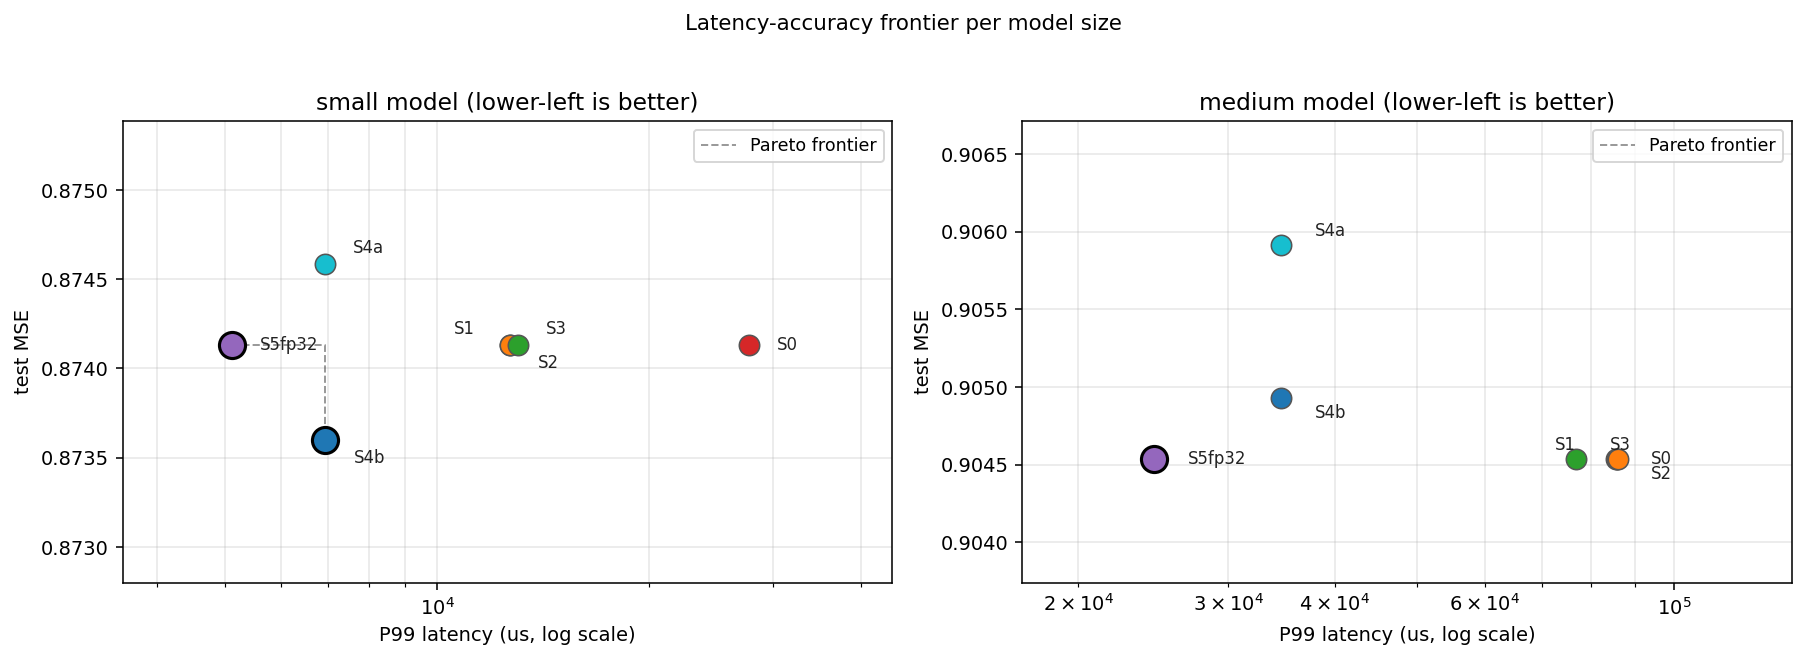
\includegraphics[width=\columnwidth]{pareto.png}
\caption{Latency--accuracy frontier per model size: P99 latency (log-$x$, $\mu$s) vs test MSE (linear-$y$). Lower-left is better. The dashed step line is the Pareto frontier within each cluster (left-to-right: keep only points whose MSE is the lowest observed so far); Pareto-optimal points are drawn with thicker borders. On small (left), Stage~5 FP32 SIMD wins on latency and Stage~4b wins on MSE, so both are Pareto-optimal. On medium (right), Stage~5 FP32 SIMD strictly dominates every other configuration.}
\label{fig:pareto}
\end{figure}

\section{Discussion}
\label{sec:discussion}

\subsection{What worked}

Three optimizations delivered measurable wins.
\emph{Preallocation} (Stage~1) is the highest-leverage optimization on small models: roughly fifty lines of C++ replace per-call \texttt{std::vector} constructions with a single contiguous activation pool, recovering $2.18\times$ P99 with no accuracy risk and no change to numerical results.
\textbf{For any latency-sensitive deployment of a sub-million-parameter model, this should be the first optimization implemented}, and other optimizations measured against it rather than against the naive baseline.
\emph{Cache tile-blocking} (Stage~3) is a clean medium-model win when the FFN intermediate exceeds L1; the $10.5\%$ P99 reduction on medium tracks the L1-miss rate reduction confirmed by \texttt{perf} counters.
\emph{INT8 with min/max histogram calibration} preserves accuracy below the noise floor of the test set itself (under $0.2\%$ absolute MSE drift), with two orders of magnitude of margin against the conventional $5\%$ production threshold.

\subsection{What didn't}

Two stages produced null or negative results, and one comparison target proved unrealistic.
\emph{Fusion B} (LayerNorm + Linear, Stage~2) was $1.00\times$ on both sizes: the intermediate it eliminates (48~KB on small, 72~KB on medium) was already L2-resident, so fusion removed memory traffic that was not on the critical path.
\emph{Tiling on small} (Stage~3) regressed $2.7\%$ relative to Stage~2; the small model's matrices fit comfortably in L2 and the tile-setup overhead is unrecouped when there is no cache pressure to relieve.
Finally, the informal benchmark ``P99 one order of magnitude below PyTorch eager'' was not met: eager's small-model P99 is 4.24~ms, our best engine (Stage~5 FP32 SIMD) reached 5.11~ms, a $1.21\times$ \emph{regression}.
A two-thousand-line hand-rolled engine does not catch MKL/oneDNN-backed eager paths that have been tuned shape-by-shape for years.

\subsection{Methodology lessons}

Three methodology observations emerged that are not specific to Transformer inference and may transfer to any tail-latency study.
First, sample size matters more than rig isolation: going from 500 to 100{,}000 iterations exposed a $540\times$ wider P99 $-$ P50 gap on Stage~0 small.
A clean rig with too few samples is worse than a noisy rig with many samples, because the noisy rig is honestly noisy while the few-sample-clean-rig is silently censored.
Second, Intel Turbo introduces a roughly $1.6\times$ P50 bias on this hardware: numbers reported on production hardware with turbo enabled will be approximately $60\%$ faster than ours, and absolute latency claims must specify rig conditions.
The \emph{ratios} between stages should remain stable across hardware, but absolute claims do not.
Third, Python tail latency is a phenomenon distinct from CPU compute.
The roughly 3~ms P99 $-$ P50 gap visible in every Python-resident baseline (PyTorch eager, TorchScript, ONNX Runtime, NumPy) is the cost of cyclic garbage collection and binding-layer object allocation, not OS jitter or compute variance: the rig's noise floor is 17~ns.
A team optimizing a Python serving stack will not close this gap by changing models; they will close it by leaving Python.

\subsection{Where this leaves us vs ONNX Runtime}

After Stage~5 FP32 SIMD, our engine reaches $1.31\times$ of ORT's P99 on the small model (5.11 vs 3.89~ms), down from $14\times$ at Stage~0.
The $11\times$ gap closure tracks cleanly to identifiable mechanisms: Stage~1 eliminated $2\times$ from the allocator tail; Stage~4 eliminated another $\sim$$2\times$ from the FP32 working set spilling to L2; Stage~5 FP32 SIMD eliminated another $\sim$$2.5\times$ from the inner-loop arithmetic.

The remaining $1.31\times$/$2.30\times$ to ORT reflects engineering investment we did not match: ORT's MLAS uses larger register-tile microkernels with more accumulators, per-($M, K, N$)-shape autotuned blocking, and (for INT8 paths) AVX-VNNI dispatch.

\section{Impact}
\label{sec:impact}

\paragraph{Deployment guidance.}
Three actionable recommendations follow directly from the ablation.
(1)~\textbf{Preallocate first.}~For any latency-sensitive deployment of a sub-million-parameter model, a single contiguous activation pool ($\approx$50 lines of C++) recovers $2.18\times$ P99 with zero accuracy risk, and every subsequent optimization should be measured against the preallocated baseline rather than the naive one.
(2)~\textbf{Per-channel INT8 is the production default} for this class of workload: it preserves test MSE within $0.06\%$ of FP32 (two orders of magnitude inside the conventional $5\%$ threshold) while delivering an $\approx$$4\times$ small-model and $\approx$$2.5\times$ medium-model speedup over scalar tiled FP32, and its P99--P50 gap is tighter than its per-tensor counterpart.
(3)~\textbf{Sub-millisecond P99.9 SLOs require leaving Python.}~Every Python-resident baseline (PyTorch eager, TorchScript, ONNX Runtime via its Python binding, NumPy) shows a 3~ms P99--P50 tail on small driven by cyclic garbage collection and binding-layer object allocation; the rig's noise floor is 17~ns, so this is not OS jitter and will not close by changing models.

\paragraph{Methodology transfer.}
Two observations generalize beyond Transformer inference to any tail-latency study.
First, \textbf{at least 10{,}000 iterations per configuration} should be regarded as a practical floor for any study claiming P99 numbers; our 500-iteration pilot underestimated the P99--P50 gap by $540\times$ relative to the 100K-iteration ground truth.
Second, \textbf{the rig state belongs inside the data, not the methods section}: recording \texttt{isolcpus}, \texttt{no\_turbo}, and \texttt{perf\_paranoia} in every CSV header makes any anomaly traceable, and lets a future reader detect a compromised measurement without re-running.

\paragraph{Conceptual.}
The most counterintuitive finding is that \textbf{scalar INT8 quantization helps medium models more than small models} ($2.22\times$ vs $1.88\times$ speedup over scalar tiled FP32), which inverts the common assumption that quantization is a ``small-model trick.''
The mechanism is L1/L2 cache fit, not arithmetic: when the FP32 working set fits in L1, INT8 saves no traffic; when it spills to L2 or DRAM, the $4\times$ working-set reduction is what buys the speedup.
This reframes how a practitioner should reach for quantization: not as a fallback when a model is too slow, but as a deliberate intervention when the FP32 working set crosses a cache boundary.

\section{Limitations}
\label{sec:limitations}

All measurements are on a single CPU (Intel Alder Lake P-core with AVX-VNNI), at batch size 1, without KV cache, on an encoder-only architecture at sequence length 96; absolute numbers will differ on AMD Zen, ARM, or pre-Alder-Lake Intel, though stage-to-stage \emph{ratios} should remain stable.
Accuracy is evaluated on ETTh1 only, so quantization MSE drift is not characterized on other distributions.
The size-dependent crossover is identified from two model scales (260K and 1.9M parameters), not a sweep: a transition exists somewhere in this interval, but two points do not pin its location.
Test MSE 0.874/0.905 reflects the published vanilla-Transformer ceiling on ETTh1 (Informer at 0.941~\citep{nie2023patchtst}), not an implementation defect; the latency findings are independent of forecasting accuracy.
Finally, bootstrap CIs assume sample independence, but adjacent iterations have short-range serial correlation from L2 and TLB warm-up; the CIs lean conservative and should not be used to claim significance for sub-microsecond deltas.

\section{Future Work}
\label{sec:future}

The most plausible path to closing the remaining $2.30\times$ gap to ORT on medium is \textbf{Stage~5 INT8 SIMD} (VNNI \texttt{\_mm256\_dpbusd\_avx\_epi32} or the non-VNNI \texttt{\_mm256\_maddubs\_epi16} + \texttt{\_mm256\_madd\_epi16} chain).
A follow-on pass should also add \textbf{\texttt{perf stat} hardware-counter} data per stage, converting the bandwidth-not-arithmetic claim from inference to measurement, and replicate the ablation at \textbf{5--6 intermediate model sizes} so the cache-fit crossover is a curve rather than a two-point transition.
Beyond this, the natural extensions are \textbf{cross-platform replication} (AMD Zen, ARM Neon, Apple Silicon), \textbf{batched inference and longer sequences} (where fused attention~\citep{dao2022flashattention} starts to matter), a \textbf{Rust port} for the latency/energy comparison motivated by~\citet{pereira2021ranking}, and \textbf{head-to-head with MLAS, TVM, and OpenVINO} to isolate which fraction of the ORT gap is library-quality versus framework-overhead.

\section{Conclusion}
\label{sec:conclusion}

We presented a six-stage ablation of a hand-coded CPU inference engine for a small encoder-only Transformer, with each stage isolating one well-known optimization.
Four answers fell out of the data and two findings contradicted common intuition.

The optimization landscape \emph{does} depend on model size, cleanly and between 365K and 1.9M parameters: preallocation buys $2.18\times$ P99 on small and nothing on medium, while cache tiling does the inverse (it costs $2.7\%$ on small but buys $10.5\%$ on medium).
INT8 quantization does \emph{not} widen the tail in a bimodal way: the P99 $-$ P50 gap is essentially unchanged after quantization on small (14 vs 15~$\mu$s) and grows only $15\%$ on medium for per-channel INT8, far below the magnitude that would constitute a saturation-driven slow path.
The hand-coded C++ engine does \emph{not} beat PyTorch eager by an order of magnitude, contrary to a folk benchmark target frequently cited for this kind of work; our best engine is in fact $1.21\times$ slower on small than PyTorch eager, because eager mode is backed by years of MKL and oneDNN kernel tuning.
Per-channel INT8 \emph{does} preserve MSE within the conventional $5\%$ production threshold by two orders of magnitude ($0.04\%$ degradation on medium) and is also tied with per-tensor on speed while exhibiting a tighter tail.

Two findings emerged that contradict common intuition.
First, sample-size sensitivity is methodologically central: 500-sample latency studies systematically under-report tail latency by orders of magnitude, and 10K samples per configuration should be regarded as a practical floor for any tail study claiming P99 numbers.
Second, scalar INT8 quantization helped the medium model more than the small one ($2.22\times$ versus $1.88\times$ speedup), inverting the common assumption that quantization is a small-model trick.
The mechanism is L1/L2 cache fit rather than arithmetic throughput: INT8's $4\times$ working-set reduction matters more when the FP32 working set genuinely overflows the cache it occupies.

The narrowly-scoped contribution of this work is not a faster Transformer engine.
\textbf{It is an honest decomposition of \emph{where} P99 latency comes from in a small-Transformer CPU inference path}, broken out by model size, with every claim independently reproducible from the recorded 100{,}000-sample CSVs and the rig configuration that each CSV's header preserves.

\bibliography{references}
\bibliographystyle{icml2026}

\end{document}
